\section{Entwurfsumentscheidungen}

\subsection{JSON Converter}
    \subsubsection{Frontend}
    % TODO Alessandro
    bla
    \subsubsection{API}
        \begin{figure}[H]
            \label{API}
            \centerline{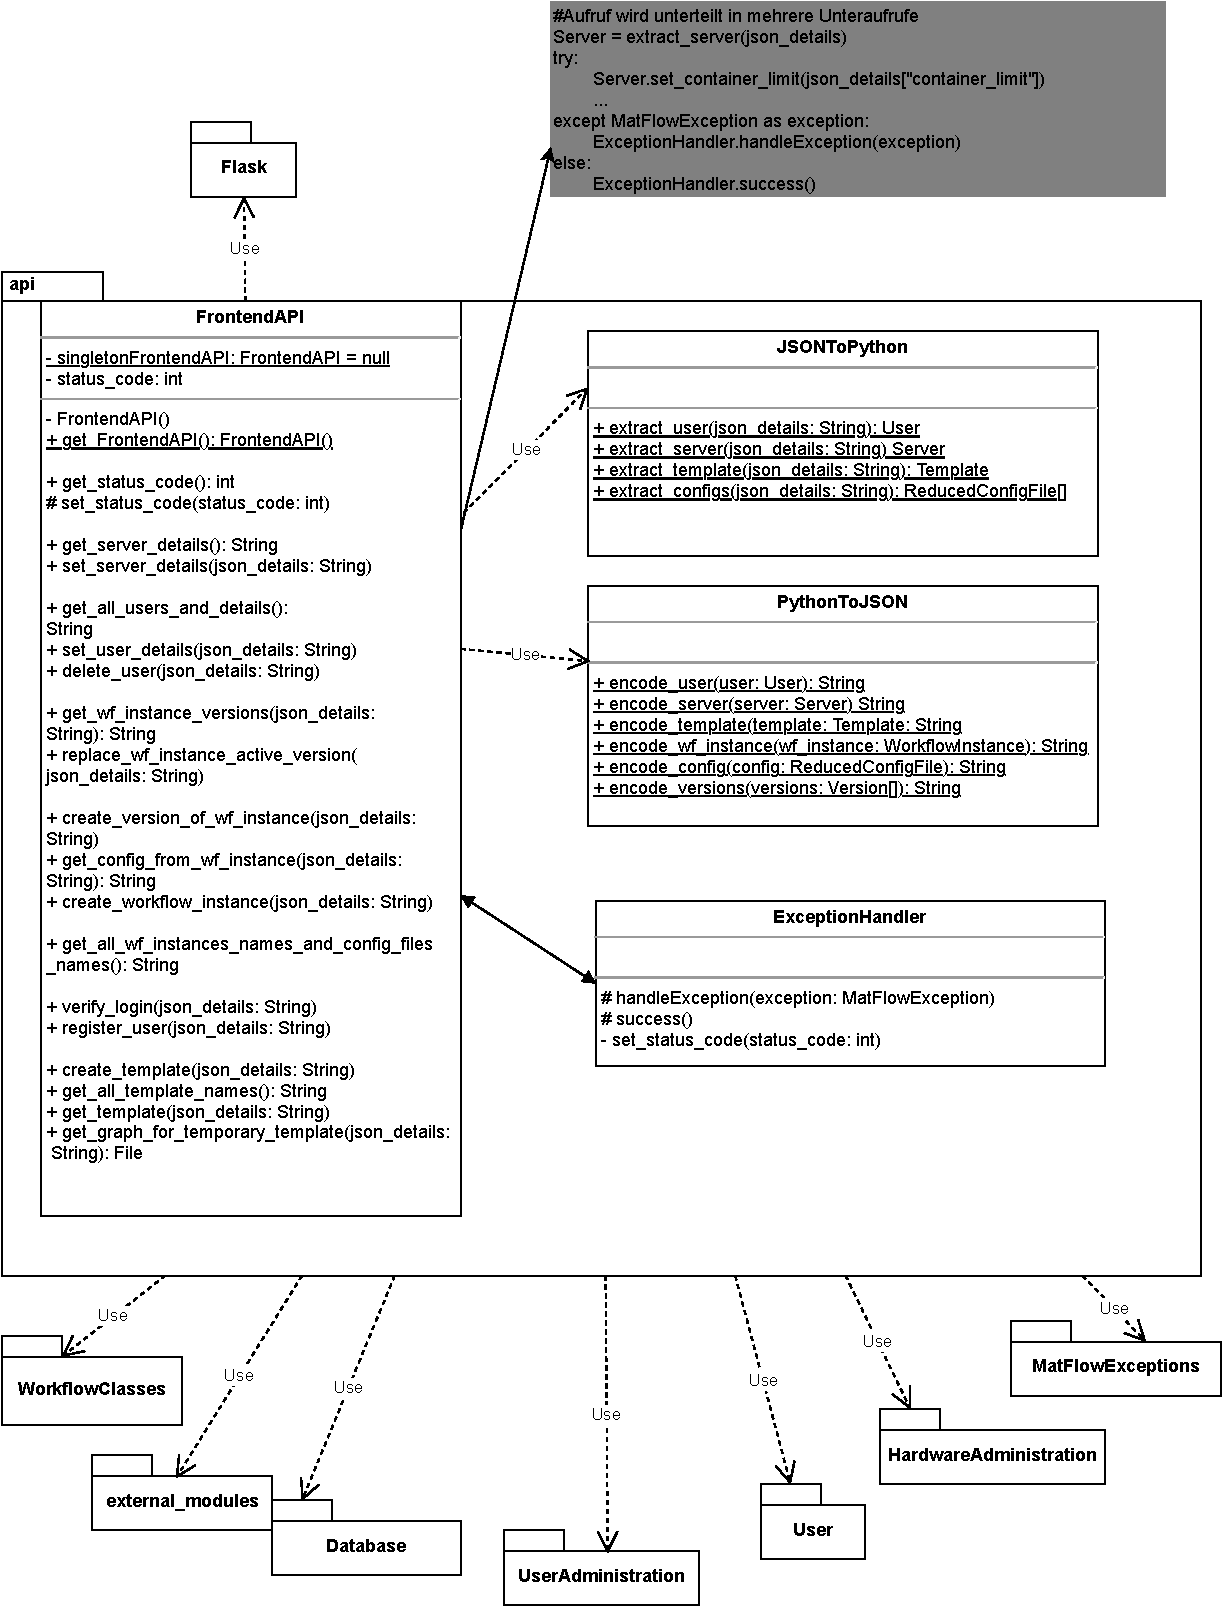
\includegraphics[scale=0.5]{res/api.drawio.pdf}}
            \caption{API package}
        \end{figure}
        \vspace{0.3in}
        Im Backend sind auch analog zum Frontend zwei JSON Converter(jewils von und zu) vorhanden.
        Diese Entwurfsentscheidung wurde aber verworfen, da sie das Kapselungsprinzip verletzt.
        Von nun an sind alle in den Converter vorhandenen Methoden direkt als Klassen- (von JSON)
        oder Objektmethoden (zu JSON) direkt in den jeweiligen Klassen implementiert. Als Beispiel: 
        encode\texttt{\_}template(template: Template) und extract\texttt{\_}template(json\texttt{\_}details: String): Template
        sind nun als encode\texttt{\_}template(self): str und \texttt{\@}classmethod extract\texttt{\_}template: Template 
        in Template vorhanden.    


\subsection{JSON Status Code}
Wie man auch in der \nameref{API} sieht, ist die Bereitstellung eines Status Codes bei einem request an die API nicht eindeutig
dem Entwurf zu entnehmen, deswegen hier noch einmal eine saubere Erläuterung:
Es wird bei einer Anfrage an die API diese Anfrage durchgeführt. Je nachdem ob sie nicht erfolgreich war (MatFlowException 
geworfen, spezieller Status Code vorhanden) oder doch erfolgreich war (success Status Code und eventuell Daten vorhanden) 
wird in der Klasse ExceptionHandler die Antwort in json gebaut und an den Client zurück geschickt. 
Der Client bekommt also \textbf{immer} eine Antwort mit einem json response body, indem sich der status code befindet. 
Es handelt sich hier also nur um eine Anlehnung an die bereits etablierten HTTP Status Codes.

\subsection{Authentifizierung} \label{Cookie}
Im Frontend kann man theoretisch unabhängig der User Privilegien mittels URL Manipulation auf alle 
Seiten zugreifen. Um dies zu verhindern, wird im Frontend ein einzigartiges Cookie mit der Anfrage an die Frontend
API geschickt, die dann ??
% TODO Alessandro
% TODO Nils dann Entwurf ändern und neues Bild posten

%TODO an alle: Entwurfsänderungen hinzufügen